\subsection{Schutzmechanismen}


\subsubsection{Adversarial Training}

In der Abbildung \ref{fig:Evaluierungspipeline} ist der Iterationsschritt der Evaluierungspipeline ersichtlich, die Pipeline wird dabei x male verwendet, was wiederum heisst, dass die Robustifizierung ebenfalls x mal geschieht. 

\begin{figure}[H]
    \centering
    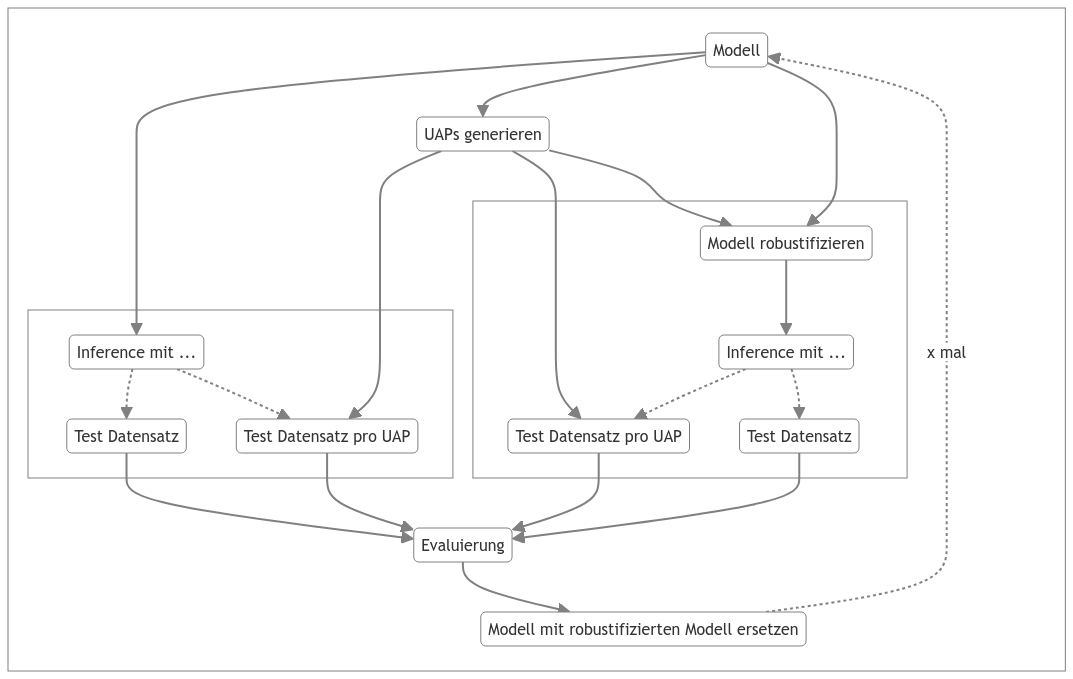
\includegraphics[width=\linewidth]{01-images/04-methodik/pipeline-robustifizierung.png}
    \caption{Übersicht der Evaluierungspipeline}
    \label{fig:Evaluierungspipeline}
\end{figure}

\begin{itemize}
    \item Modell: Startpunkt der Pipeline, bzw. unser trainiertes Modell auf unseren Datensatz. 
    \item UAPs generieren: \acrlong{uap} werden generiert, um das Modell zu robustifizieren
    \item Modell robustifizieren: Adversarial Training
    \item Inferenz mit...: Geschieht durch zwei Parallele Wege, 
        \begin{itemize}
            \item einer führt zur Inferenz mit dem ursprünglichen Modell, jeweils für den Testdatensastz mit und ohne \acrshort{uap}
            \item der andere Weg führt zur Inferenz mit dem robustifizierten Modell
        \end{itemize}
    \item Evaluierung: Im Evaluierungsschritt sind vier Pakete durch die Inferenz enthalten, die miteinander verglichen werden. 
\end{itemize}